\newSec[Flight]{Analyse realer Flugdaten}{2}

\newSec[FlightData]{Datenbasis}{3}
Dieses Kapitel zeigt die verschiedenen Daten des Flugs, um diese in der nachfolgenden Analyse einordnen zu können.

Der gezeigte Datensatz enthält zwei Flüge, welche naheinander aufgenommen wurden. Aus diesen Daten wurden irrelevante Einträge zwischen den Flügen entfernt. Durch diesen Eingriff wurde der berechnete Verlauf des zweiten Fluges nicht beeinflusst, da die Status des \Quad\ zu geeigneten Zeitpunkten zurückgesetzt werden.

Der vom Zustandsautomaten der \Ar\ einnehmbare ZustandIDs sind im \CodePkg{ardrone\_autonomy} wie folgt definiert:
\begin{table}[!ht]
\begin{tabular}{ll}
StatusID & Status-Text    \\ \hline
0        & Unknown        \\
1        & Init           \\
2        & Landed         \\
3        & Flying         \\
4        & Hovering       \\
5        & Test           \\
6        & Taking off     \\
7        & Goto Fix Point \\
8        & Landing        \\
9        & Looping       
\end{tabular}
\end{table}
\FloatBarrier
Aus den Flugversuchen zeigte sich, dass StatusID 6 (\textit{Taking off}) nicht gesendet wird. Stattdessen wird StatusID 7 (\textit{Goto Fix Point}) unmittelbar nach der \textit{Takeoff}-Message eingenommen. StatusID 8 (\textit{Landing}) wird durch StatusID 9 (\textit{Looping}) abgebildet. 


\begin{figure}[ht!]
\vspace{0.25cm}
\begin{center}
\fbox{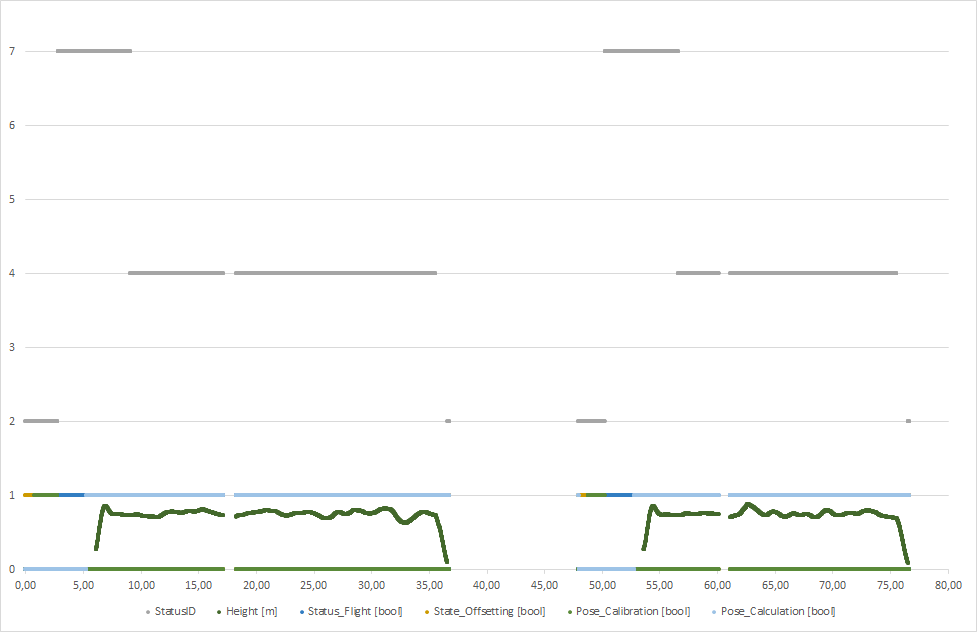
\includegraphics[width=15cm]{Pictures/TestFlight Status Flags Height.png}}
\caption{Testflug: StatusID, Flags und Höhenprofil}
\label{fig:FlightStatus}
\end{center}

\vspace{0.25cm}
Um die Aussagekraft der Graphik zu gewährleisten wurde die Ordinatenachse lediglich bis zum Wert 7 abgebildet. Hierdurch wird die StatusID der Landephase ausgespart.
\end{figure}

Aus den Daten kann eine \textit{ground truth} für die Position der z-Achse entnommen werden. Diese Daten stammen von dem auf den Untergrund gerichteten Ultraschall-Sensor.\\
Eine Genaue Abschätzung der Korrektheit dieser Daten lässt sich nicht aus Vergleichsdaten belegen. Die Genauigkeit des Untraschall-Sensors kann jedoch als höher angenommen werden als die der berechneten Pose.


\FloatBarrier
\newSec[FlightProcess]{Verlauf des Fluges}{3}

\missing[Hier Abb 18 detailliert geschreiben. Besonders auf Flags eingehen.]







\newSec[FlightAnalysisLeak]{Lecks der Datenübertragung}{3}
Aus den Daten, aufgetragen in \refImg{fig:FlightStatus}, und weiteren Testflugen zeigt sich, dass die Verbindung zwischen dem Host-PC und dem \Quad\ anfällig für Verbindungsunterbrechnungen ist. Während diesen Unterbrechnungen werden für einen Zeitraum von etwa einer Sekunde keine Nachrichten übermittelt. 

Die entwickelte Software sieht für diese Fälle keine Interpolation der Daten vor. Hieraus entstehen Sprünge in den berechneten Daten. Hier können als Beispiel \refImg{fig:FlightPoseVel} und \refImg{} jeweils für die Zeitbereiche um 17 Sekunden und 61 Sekunden herangezogen werden.
\missing[Bild der berechneten Pose referenzieren.]







